\begin{center}
    {\LARGE \textbf{2020物理化学}} \\[2ex]
    {\large 时量180分钟 \quad 满分150分}
\end{center}

\vspace{0.5cm}
\noindent\textbf{注意事项:}
\begin{enumerate}[label=\arabic*., parsep=0pt, itemsep=0pt]
    \item 答题前,考生先将自己的姓名、学号、考场号、座位号填写在答题卡上,将条形码准确粘贴在考生信息条形码粘贴区。
    \item 考试结束后,将本试卷与答题纸一并收回。
    \item 回答各个问题时,将答案写在答题纸上,写在本试卷上无效。
\end{enumerate}

\vspace{0.5cm}
\noindent\textbf{一、选择题(30 pts.)}

\begin{enumerate}[label=\arabic*., itemsep=1.5ex]
    \item 某化学反应在恒压、绝热和只作体积功的条件下进行，体系的温度由$T_1$升高到$T_2$，则此过程的焓变：
    \begin{tasks}(4)
        \task 小于零
        \task 等于零
        \task 大于零
        \task 不能确定
    \end{tasks}
    \item 固体六氟化铀的蒸气压$p$与$T$的关系为$\lg(p/\mathrm{Pa})=10.65-2560/(T/K)$，则其平均升华热为：
    \begin{tasks}(4)
        \task $2.128\mathrm{kJ\cdot mol^{-1}}$
        \task $49.02\mathrm{kJ\cdot mol^{-1}}$
        \task $9.242\mathrm{kJ\cdot mol^{-1}}$
        \task $10.33\mathrm{kJ\cdot mol^{-1}}$
    \end{tasks}
    \item 理想气体从状态Ⅰ经自由膨胀到状态Ⅱ，可用哪个热力学判据来判断该过程的自发性？
    \begin{tasks}(4)
        \task $\Delta H$
        \task $\Delta G$
        \task $\Delta S$
        \task $\Delta U$
    \end{tasks}
    \item 已知$373.15K$时，液体$\ce{A}$的饱和蒸气压为$133.32\mathrm{kPa}$，另一液体$\ce{B}$可与$\ce{A}$构成理想液体混合物，当$\ce{A}$在溶液中的物质的量分数为$1/2$时，$\ce{A}$在气相中物质质量分数为$2/3$时，则在$373.15K$时，液体$\ce{B}$的饱和蒸气压应为：
    \begin{tasks}(4)
        \task $66.66\mathrm{kPa}$
        \task $88.88\mathrm{kPa}$
        \task $133.32\mathrm{kPa}$
        \task $266.64\mathrm{kPa}$
    \end{tasks}
    \item $598.15K$时，与汞的摩尔分数为$0.497$的汞齐呈平衡的气相中。汞的蒸汽压为纯水在该温度下的饱和蒸汽压的$43.3\%$，汞在该汞齐的活度因子为$\gamma_{\mathrm{Hg}}$：
    \begin{tasks}(4)
        \task $1.15$
        \task $0.87$
        \task $0.50$
        \task $0.43$
    \end{tasks}
    \item 在一定的温度下，一定量$\ce{PCl_{3}(g)}$的在一密闭容器中达到分解平衡。若往容器中充入氮气，实体系的压力增加一倍(体积不变)，则$\ce{PCl_{3}}$的解离度将为
    \begin{tasks}(4)
        \task 增加
        \task 减少
        \task 不变
        \task 不定
    \end{tasks}
    \item 在等压下，无论用什么过程进行一个$\ce{A + B = C}$的反应，若$\Delta_rH_m>0$，则该反应一定为：
    \begin{tasks}(2)
        \task 吸热反应
        \task 放热反应
        \task 无热量变化
        \task 视反应过程而定
    \end{tasks}
    \item 反应$\ce{A(g) + 2B(g) -> 2D(g)}$在温度$T$时的$K_p^\ominus=1$，若温度恒定为$T$，在一真空容器中通入$\ce{A}$、$\ce{B}$、$\ce{D}$三种理想气体，他们的分压恰好皆为$101.3\mathrm{kPa}$。在此条件下，反应将
    \begin{tasks}(4)
        \task 从右向左进行
        \task 从左向右进行
        \task 处于平衡状态
        \task 无法判断
    \end{tasks}
    \item $\ce{NaCl}$水溶液和纯水经半透膜达成渗透平衡时，该体系的自由度是：
    \begin{tasks}(4)
        \task $1$
        \task $2$
        \task $3$
        \task $4$
    \end{tasks}
    \item 如果反应$\ce{2A + B=2D}$的速率可表示为：
    \[
    r = -\frac{1}{2}\frac{dc_A}{dt} = -\frac{dc_B}{dt} = \frac{1}{2}\frac{dc_D}{dt}
    \]
    则其反应分子数为：
    \begin{tasks}(4)
        \task 单分子
        \task 双分子
        \task 三分子
        \task 不能确定
    \end{tasks}
    \item 放射性的$\ce{Pb^{201}}$半衰期为$8\mathrm{h}$，$1\mathrm{g}$放射性$\ce{Pb^{201}}$在$24\mathrm{h}$后还剩下：
    \begin{tasks}(4)
        \task $1/8\mathrm{g}$
        \task $1/4\mathrm{g}$
        \task $1/3\mathrm{g}$
        \task $1/2\mathrm{g}$
    \end{tasks}
    \item 根据碰撞理论，温度增加，反应速率提高的主要原因是：
    \begin{tasks}(2)
        \task 活化能降低
        \task 碰撞频率提高
        \task 活化分子所占比例增加
        \task 碰撞数增加
    \end{tasks}
    \item $298K$下，当$\ce{H_{2}SO_{4}}$溶液的浓度从$0.01\mathrm{mol\cdot kg^{-1}}$增加到$0.1\mathrm{mol\cdot kg^{-1}}$时，其电导率$k$和摩尔电导率$\Lambda_m$将：
    \begin{tasks}(4)
        \task $k$减小，$\Lambda_m$增加
        \task $k$增加，$\Lambda_m$增加
        \task $k$减小，$\Lambda_m$减小
        \task $k$增加，$\Lambda_m$减小
    \end{tasks}
    \item 电解金属盐的水溶液时，在阴极上：
    \begin{tasks}(1)
        \task 还原电势愈正的粒子愈容易析出
        \task 还原电势与其超电势之代数和愈正的粒子愈容易析出
        \task 还原电势愈负的粒子愈容易析出
        \task 还原电势与其超电势之代数和愈负的粒子愈容易析出
    \end{tasks}
    \item 下述体系中的组分，选择假想标准态的是：
    \begin{tasks}(2)
        \task 理想溶液中的组分$\ce{B}$
        \task 理想混合气体中的组分$\ce{B}$
        \task 非理想溶液中的溶剂
        \task 稀溶液中的溶质$\ce{B}$
    \end{tasks}
\end{enumerate}

\vspace{0.5cm}
\noindent\textbf{二、填空题(10 pts.)}

\begin{enumerate}[label=\arabic*., itemsep=1.5ex]
    \item 在晴朗的白昼，由于蓝光波长\underline{\hspace{2cm}}，\underline{\hspace{2cm}}作用显著，所以天空成蔚蓝色。
    \item 明矾净水的主要原理是溶胶的\underline{\hspace{2cm}}作用。
    \item 乳状液可分$\ce{O/W}$型和$\ce{W/O}$型。一般来说，若乳化剂是憎水性的，形成的是\underline{\hspace{1cm}}型乳状液；若乳化剂是亲水性的，形成的是\underline{\hspace{1cm}}型乳状液。
    \item 植物的叶子一般是憎水性的，所以在配置农药时常常要加\underline{\hspace{2cm}}，以增加药液对植物表面的润湿程度，是药液能在植物叶子上铺展。
    \item 分子的平动、转动和振动的能级间隔的大小顺序是\underline{\hspace{4cm}}。
\end{enumerate}

\vspace{0.5cm}
\noindent\textbf{三、计算题(20 pts.)}

$1\mathrm{mol}$理想气体在$122K$等温的情况下反抗恒定外压从$10\mathrm{dm}^3$膨胀到终态，已知该过程体系的熵变为$19.14\mathrm{J\cdot K^{-1}}$，
\begin{enumerate}[label=(\arabic*), itemsep=1ex]
    \item 求该膨胀过程体系反抗的外压$p_e$，终态的体积$V_2$；
    \item 计算$\Delta U$，$\Delta H$，$\Delta F$，$\Delta G$，$\Delta S_{\text{环}}$，$\Delta S_{\text{孤立}}$；
    \item 适用何种热力学判据判断该过程的变化性质并判断之。
\end{enumerate}

\vspace{0.5cm}
\noindent\textbf{四、计算题(15 pts.)}

$101.325\mathrm{kPa}$下，纯苯的凝固点为$278.55K$，现有$0.223\mathrm{g}$苯甲酸溶于$4.4\mathrm{g}$苯中，该体系于$277.62K$开始结晶。已知苯的熔化热为$9.89\mathrm{kJ\cdot mol^{-1}}$，苯甲酸分子的摩尔质量为$122.1\mathrm{g\cdot mol^{-1}}$。
\begin{enumerate}[label=(\arabic*), itemsep=1ex]
    \item 试计算苯甲酸的相对分子质量。
    \item 请对计算结果给予讨论。
\end{enumerate}

\vspace{0.5cm}
\noindent\textbf{五、计算题(15 pts.)}

将固体$\ce{NaHCO_{3}}$放入真空容器中会发生分解反应：
\[
\ce{2NaHCO_{3}(s) -> Na_{2}CO_{3}(s) + H_{2}O(g) + CO_{2}(g)}
\]
求：
\begin{enumerate}[label=(\arabic*), itemsep=1ex]
    \item $25^\circ C$，该平衡体系的总压为多少？
    \item 若平衡总压为$101.325\mathrm{kPa}$，该体系的温度为多少？
\end{enumerate}
已知下列数据($\Delta_fH_m^\ominus$，$S_m^\ominus$均为$298K$时的数据，且受温度影响可忽略)：
\begin{center}
\begin{tabular}{lcccc}
\hline
 & $\ce{NaHCO3(s)}$ & $\ce{Na2CO3(s)}$ & $\ce{CO2(g)}$ & $\ce{H2O(g)}$ \\
\hline
$\Delta_f H_m^\ominus\,/\,\mathrm{kJ\,mol^{-1}}$ & $-947.7$ & $-1130.9$ & $-393.5$ & $-241.8$ \\
$S_m^\ominus\,/\,\mathrm{J\,K^{-1}\,mol^{-1}}$ & $102.1$ & $136.6$ & $213.6$ & $188.7$ \\
\hline
\end{tabular}
\end{center}

\vspace{0.5cm}
\noindent\textbf{六、计算题(20 pts.)}

已知两组分$\ce{A}$和$\ce{B}$体系的相图如下：

\begin{figure}[htbp]
    \centering
    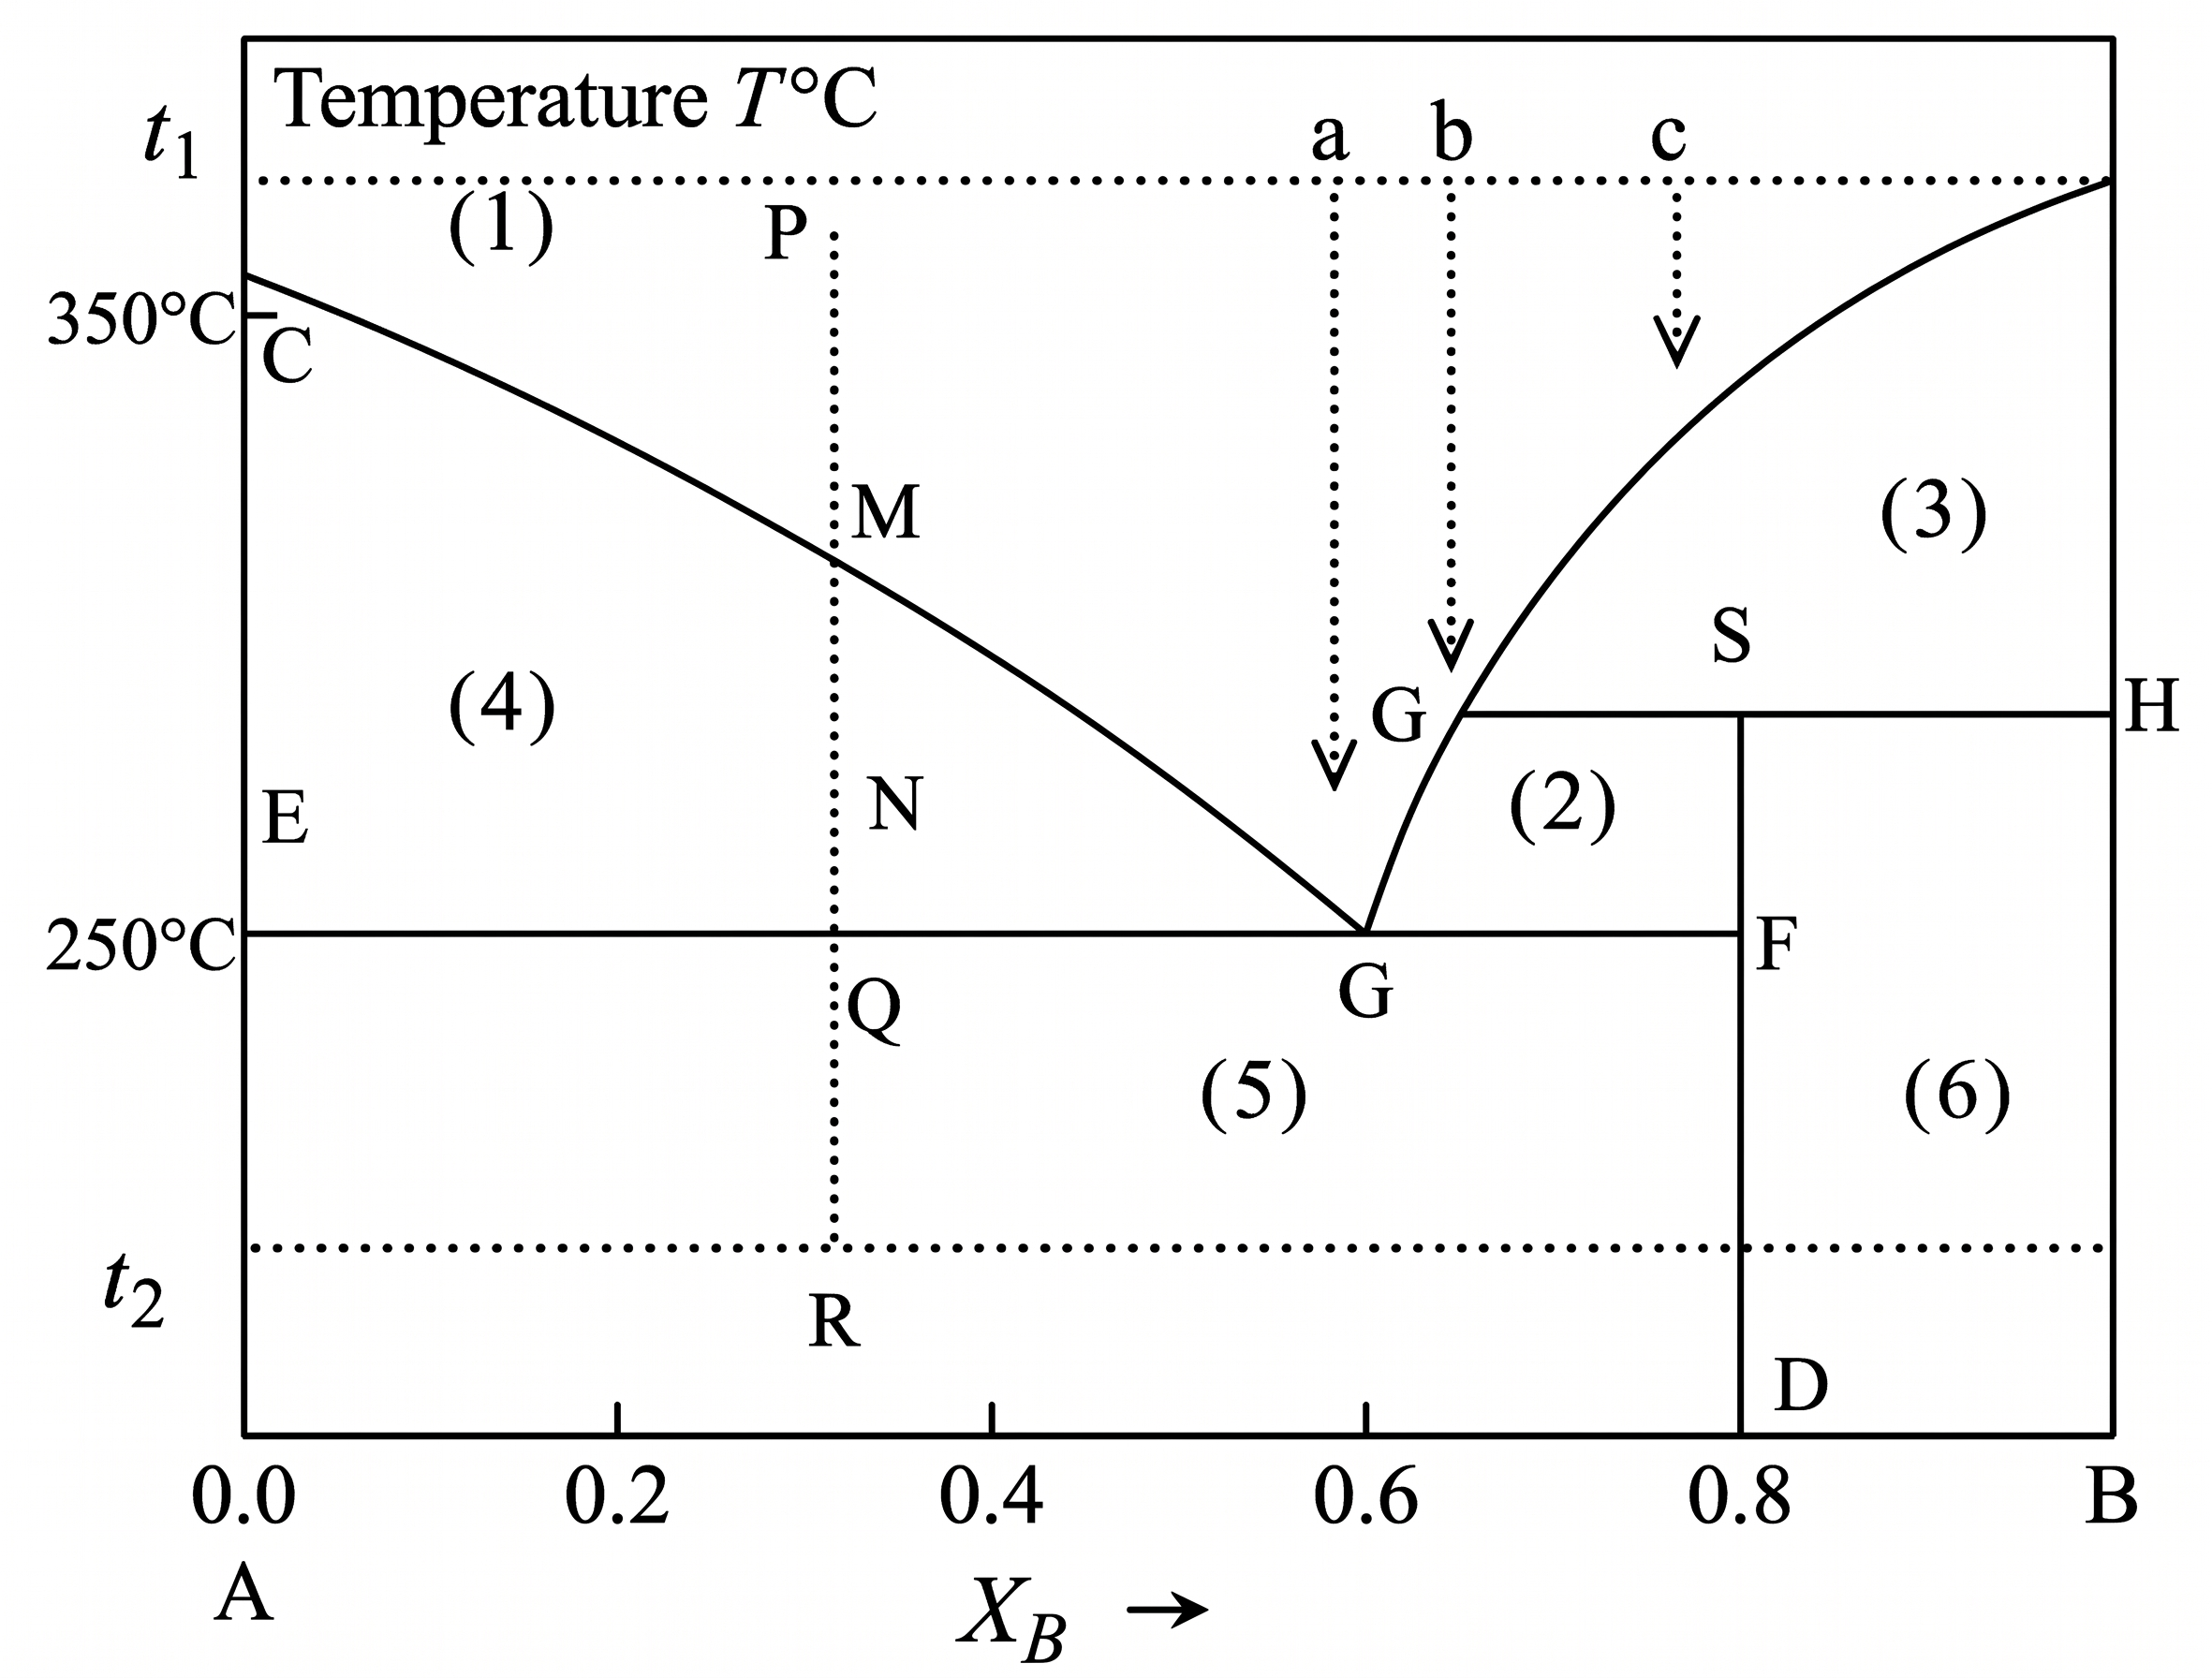
\includegraphics[width=0.6\textwidth]{./Figure/P_2020_6}

\end{figure}

\begin{enumerate}[label=(\arabic*), itemsep=1ex]
    \item 画出$p$点表示的体系由$t_1$温度冷却到$t_2$的步冷曲线；
    \item 标出各相区的相态和自由度，$\ce{EF}$水平线，$\ce{GH}$及$\ce{SD}$垂直线的相数和自由度；
    \item 使体系$\ce{P}$降温，说明达到$\ce{M}$，$\ce{N}$，$\ce{Q}$，$\ce{R}$点时体系的相态和相数；
    \item $1\mathrm{kg}$含$\ce{B}$ $40\%$的熔化物降温到$t_1$时可以得到什么物质？请计算其质量。
\end{enumerate}

\vspace{0.5cm}
\noindent\textbf{七、计算题(15 pts.)}

在高温时，醋酸的分解反应按下式进行：
\[
\ce{CH_{3}COOH ->[k_1] CH_{4} + CO_{2}} \quad \ce{CH_{3}COOH ->[k_2] CH_{2}=CO + H_{2}O}
\]
在$1189K$时，$k_1=3.74s^{-1}$，$k_2=4.65s^{-1}$，求：
\begin{enumerate}[label=(\arabic*), itemsep=1ex]
    \item 醋酸分解掉$99\%$所需时间
    \item 这时所能得到的$\ce{CH_{2}=CO}$的产量(以醋酸分解的百分数表示)
    \item 怎样才能有效的提高$\ce{CH_{4}}$的产量？
\end{enumerate}

\vspace{0.5cm}
\noindent\textbf{八、计算题(15 pts.)}

反应$\ce{Zn(s) + CuSO_{4}(a=1) -> Cu(s) + ZnSO_{4}(a=1)}$在电池中进行，$15^\circ C$时，测得$E=1.0934\mathrm{V}$，电池的温度系数$\left(\frac{\partial E}{\partial T}\right)_p=-4.29\times10^{-4}\mathrm{V\cdot K^{-1}}$
\begin{enumerate}[label=(\arabic*), itemsep=1ex]
    \item 写出电池表示式和电极反应式；
    \item 求电池可逆输出$2\mathrm{F}$电量时的$\Delta_rG_m^\ominus$，$\Delta_rS_m^\ominus$，$\Delta_rH_m^\ominus$和$Q_r$；
    \item 如果电池是在$75^\circ C$时可逆输出$2\mathrm{F}$电量，求电池输出电功若干；
\end{enumerate}

\vspace{0.5cm}
\noindent\textbf{九、简答题(10 pts.)}

\begin{enumerate}[label=\arabic*., itemsep=1.5ex]
    \item 什么样的电池才是可逆电池？
    \item 请简述水的冰点和三相点的热力学定义的区别。
\end{enumerate}